\chapter{Research Avenues}
\label{ch:researchavenues}
% ##################################################################################################################

\hfill \textbf{Authors:} Kai Nagel, Kay W.\ Axhausen, Benjamin Kickhöfer, Andreas Horni

\begin{center} 
\includegraphics[width=0.3\textwidth, angle=0]{frontmatter/figures/MATSimBook} \end{center}

% ##################################################################################################################
The on-going work and the interest documented in the many scenarios shows 
that the system has not exhausted its possibilities as a platform for research on it and with it. 
This chapter wants to highlight some of them for further discussion and maybe action. 

% ##################################################################################################################
\section{MATSim and Agents}

% Q-learning: learn utility for each state-action pair
%
% utility learning: learn utility for each state
%
% difference: In the second case, need to have a model about the world.  I.e. need to know which actions lead to which probabilities for the next state.

% 20.2 passive learning in a known environment

% naive: proceed until terminal state, backpropagate utility to all previous states, average over all such utility values ever collected per state

% adaptive dynamic programming: U(i) = R(i) + \sum_j M_{ij} U(j)

% where R(i) is the reward at i and M_{ij} are the transition probas 
% (recall that this is passive learning)

% I don't that that this can be sampled ... needs to solve the equations

% temporal difference (TD) learning: U(i) <-- U(i) + alpha * ( R(i) + U(j) - U(i) ) 

% 20.3 passive learning in an unknown environment

% Since TD never neede M_{ij}, it will still work as before.  Will now also 
% learn M_{ij}, but separately

% 20.4 active learning in an unknown environment

% Now M^a_{ij} (depending on the action)

% U(i) = R(i) + max_a \sum_j M^a_{ij} U(j)

% TD approach same as before

% 20.5 Exploration

% 20.6 Learning an action-value function (Q values, Q-learning)

The core \gls{matsim} architecture---where agents learn utilities for plans---was originally derived from the so-called field of \glspl{cas}.  
%
\cite{ArthurBar} addresses a coordination problem, where agents receive a payoff only when less than 60 out of 100 go to an event.  He addresses this by first generating a large number of heuristic predictors for the next round's attendance, such as ``same as in last round'' or ``trend of last four rounds''.  He next gives each agent a randomly selected handful of these strategies, so that agents in general have different sets of predictors.  Then, many rounds of the game are played, where the score of each predictor is updated based on its prediction quality, and agents act based on their currently best predictor.  Simulations demonstrate that the approach leads to successful coordination, \ie around 60\,agents show up in every round.
%
That approach in turn builds on work by \cite{PalmerEtAl_PhysicaD_1994}, who simulate a stock market, \citet{Holland_1992}, whose classifier systems have more structure than Arthur's model but have a similar model of performance learning, or \cite{AxelrodBook}, who investigates adaptive agent in the face of repeated non-cooperative games.  

\citet{ArthurBar} kept each agent's predictors fixed after initialization.  In contrast,
\citet{HraberJonesForrestEcho} simulate an artificial ecosystem, where the individual agent strategies are based on so-called genes, which are adapted over the rounds/iterations by a genetic algorithms \citep{Goldberg_1989}.

The focus of \gls{cas} is on many agents, agent interaction, and emergence. \Gls{ai} in contrast concentrated on single agents. In \gls{ai} terms, the original \gls{matsim} agents (those that do day-to-day learning) are very simple active reinforcement learning agents \citep[][Chapter 21.3]{RusselNorvig2010ArtificialIntelligence}. Since these \gls{matsim} have only one state and each plan is simply an action, the distinction between Q-learning and utility learning actually collapses, and what remains is the temporal difference learning scheme for the utility, which translated to the \gls{matsim} situation updates the score/performance/utility value of each plan every time it is selected.

That is, overall, the original \gls{matsim} system has inherited the focus on large systems, interaction, and emergence as well as the approach to strategy innovation from \gls{cas}, while the score updating rather comes from the field of \gls{ai}.

In the meantime, both \gls{ai} and the field of transport simulation have moved on, increasingly looking at agents that can react immediately, rather than having to wait for the next iteration or round.  In transport, this is sometimes called en-route or within-day replanning \citep[e.g.,][]{EmmerinkEtAl_TransResC_1995,balijepalli-2007}.

\kai{to do more}

% ##################################################################################################################
\section{Within-Day Replanning and the User Equilibrium}
\label{sec:researchavenues-withinday}
Within-day replanning, \ie the ability of the agents to respond to the immediate context is the standard mode of operation for simulation models. Note the traffic flow models in the transport domain, for example. Many agent based models travel demand of travel demand adopted the same approach (ORIENT, ORIENT/RV, MobiTOPP, Emmerink et al., \ah{cite} and all the work on intelligent transport system \kwaah{do we have more?}), but none of these aim for equilibrium in the sense adopted by \gls{matsim} carried forward from \gls{transims}. If supplied with a learning approach these within-day models should approach equilibrium after many iterations, as the agents with a suitable memory structure would avoid plans which make them worse off. This memory, which would need to be agent-specific and covering the very large set of choice options, makes the approach costly to implement. 

Still, there are context where this immediate response ability could be used within \gls{matsim} to explore the choice set more effectively, especially if the choice alternatives are limited in number and in geographic reach. Waraich et al. (200x) \kwaah{What is the best reference here?} use a localized within-day, actually within-trip search to find the best parking space around a destination. This localized search reduces the need for full iterations considerably and allows to add behavioural detail at this point, here the type of space, walking distance and parking fee trade-off. In the same spirit, Horni (2015) \ah{Gibt es da schon etwas?} employs the same approach to address crossing of signalized intersections. 

While within-day replanning can be used as described above within the framework equilibrium search, it can also be added to open up the \gls{matsim} framework to context, where such an equilibrium is inappropriate. \citet[][]{Dobler_PhDThesis_2013} used the \gls{matsim} calculated equilibrium as the starting point for his model of evacuations and the behavior of the evacuees. He also documents that his approach finds a set of executed plans, which is close to the \gls{matsim} equilibrium, but for much lower computing costs. While the benefits of an equilibrium solution in comparison with an approximation have been extensively discussed for aggregate assignment models, for \gls{matsim} the issue is, if these fast approximation could be used to speed up the overall equilibrium search; similar in spirit to start a Frank-Wolf search based on four or five incremental network loadings of the network. While aggregate assignment has possibilities to identify the routes chosen as belonging to the equilibrium, in the agent-based context research is needed to a) see, if the approach is indeed faster and b) if the resulting set of plans is unbiased by the fast initialization. 


\vfill\eject
% ##################################################################################################################
\section{Choice Set Generation}
\label{sec:choicesets}

\kai{in particular plans removal!! From Benjamin's diss:}

In the plans innovation process of the simulation, the plan with the lowest utility is removed whenever the maximum number of plans are reached for an agent. In consequence, this decreases the probability that heterogeneous plans survive and increases the probability of very similar plans. This, again, increases the likelihood that the final choice set is correlated, \ie containing only plans that are very similar to the best plan \citep[see][for a review on correlation of 
 routes]{Prato2009ChoiceModellingSurvey}.%
 %
 \footnote{
 %
 A possible solution to this problem is most likely composed of two steps:
 %
 First, more heterogeneity needs to be introduced into the choice set generation, \eg by producing very different plans.
 %
 Second, the method for plans removal needs to be based on an \gls{mnl} model where the difference in utility enters, similar to the approach of selecting plans for execution. This could be done by an implementation of a method called \gls{pathsizelogitmodel} which uses similarity measures for plans \citep[see][for a possible solution in route choice]{FrejingerBierlaire2007PathSizeLogit, BenAkivaBierlaiere1999DiscreteChoice}.
 %
 }

---

To give recommendations to other researchers: the bias in choice set generation of \gls{matsim} needs to be fixed in the near future in order to obtain valid choice sets.
%
This requires (i) the generation of more heterogeneous plans \citep[see, e.g.,][for such attempts in the \acrshort{pt} and in the car mode, respectively]{Moyo2013PhD, NagelKickhoeferJoubert2014HeterogeneousVoTsPROCEDIA}; and (ii) the implementation of a \gls{pathsizelogitmodel} in the plans removal process \citep[see, e.g.,][]{Grether2014PhD}.
%
Having obtained these valid choice sets \citep{NagelFloetteroed2009IatbrResourceInBook}, the calculation of user benefits based on the \gls{logsum} formulation is preferable.
%
\benjamin{Well, here it now depends on how we write the previous section...}
%
Using the logsum formulation with correlated choice sets requires a careful interpretation of the results. However, when looking at differences between the two states before and after a policy, this issue is unlikely to change results structurally: if the correlation remains roughly the same between the two states, the error of utility differences is small. If the correlation structure of plans changes, the error will\textemdash among other model specifications\textemdash depend on the number of iterations.
%
\benjamin{If we iterate the base case to the same iteration number as the policy case, the former will be more correlated. This would result in a underestimation of the utility changes.}
%
In that sense, one could include some approximation of the error into the analysis of results, possibly similar to Equation~(\ref{eq:ch:economicEval:logsumMaxError}). If the differences in utility levels between the two states are in the same magnitude as $\ln(P)$, it is possible that the signal of the policy effect is smaller than the noise of randomness.

% ##################################################################################################################
\section{Utility Function}
\label{sec:future-of-scoring-function}

\ah{Shortcomings of current standard \gls{matsim} utility function: activity choice (see Section~\ref{sec:alternative-functions}), curvature param, estimates, ...}

% =========================================================================================
\subsection{Alternative Functional Forms of the Utility Function}
\label{sec:alternative-functions}
The current logarithmic \gls{matsim} utility function is not suitable for modeling activity sequence choice \citet[][p.127f]{Feil_PhDThesis_2010} and \citet[][]{MATSim_Userguide_2015}. Because of its negative second derivative, \ie its concavity, the log form favors very short activities, which means that the schedule is ever filled-up with short activities, where the usually long home activities are replaced first. Since this generates completely unrealistic behavior, a new function was introduced by \citet[][p.129ff]{Feil_PhDThesis_2010}. The function was based on the asymmetrically S-shaped function proposed by \citet[][]{Joh_PhDThesis_2004}. Estimates of the new function based on the Swiss microcensus were provided. The estimation, however, suffered inherent stability issues as shown below. The function was, thus, not further developed.

% ----------------------------------------------------------
\subsubsection{Stability Issues With the S-Shaped Function}
With a fixed number of activities the log form optimum lies as far to the right as the overall budget constraint allows. 
In line with consumer theory's utility maximization, all first derivatives are equal and the unique optimum is stable.
A flexible number of activities is wandering towards zero duration as the marginal utility is largest at zero. 
Zero duration is a singularity. 
Additionally, only the activity type with the shortest typical duration will survive the optimization process.

Establishing a positive second derivative near point of origin, by using an S-shaped utility function, is a natural idea to work against this degenerated mechanism of adding more and more and ever shorter activities.
The problem of the diminishing of these activities with longer typical durations, such as home activities, remains the same, when the number of activities is flexible.
Furthermore, there are points where common system stability criteria---small perturbations only have small effects---is broken.
At such points of the optimization trajectory, for filling up the time budget, it is suddenly better to add a new activity to the convex region than to prolong an activity in the concave region.
Due to the the S-shaped function's symmetry, these points seem to fall together with the inflection points of the the bell-shaped first derivative of the S-shaped function.

% ----------------------
%\ah{Some pieces of notes:
%
% The optimization problem however, does neither have a stable optimum. An S-shaped function's first derivative is bell-shaped, \ie not bijective,
%
%The optimum is only kept, in the rare case, where the budget constraint exactly matches with all activities being at their utility function's inflection point, where the marginal utility is maximal.
%In all other cases ...
 %
%The maximum marginal utility is at the inflection point.
%
% The log forms first derivative $1/x$ is bijective.
%
%Together with the flexible number of activities, this means that there are infinitely many optima, \ie
%the time budget $T$ can be assigned to a variable number of activities in infinitely many ways representing an optimal plateau.
%
%with $N$ activities of which $m$ activities lie below injection point with first derivative $\cdot{f_0}$ and $N-m$ activities lie above injection point with first derivative $\cdot{f_1}$, 
%the total time budget $T$,
%and the infinitely small time change $dt$ 
%\begin{equation}
%m \cdot \dot{f_0}(t_0) \cdot dt = (N-m) \cdot \dot{f_1}(t_1) \cdot (T-m\cdot dt)/(N-m)
%\end{equation}
%has infinitely many solutions as $N$, $t_0$, $t_1$ are flexible; $t_0$ and $t_1$ are dependent on each other though.
%This also includes the case that activities have zero durations.
%In any case, it is very difficult to estimate such a function.
%Its behavioral suitability is another unsolved issue.
%
%\ah{ungewöhnliche Notation mit $dt$, wie schreibt man das sonst?}
%
%
%-------------
%
%consumer theory, first derivative equal -> defined clear optimization problem. 
%
%In other words, first derivatives do not need to be equal, 
%
%various combinations of activities lying above utility function injection point while others are below it are possible.
%
%This means that as long as the number of activities is flexible (degree of freedom) there exist ...
%
%The system is only stable (and optimal) if all non-zero-duration activities are exactly at inflection point of the utility function as detailed by following differentiation: 
%\begin{enumerate}
%\item All activities are in concave region (thus having equal marginal utility). Adding another activity might add additional benefit. 
%\item All activities are in convex region (thus having equal marginal utility). Removing one activity might add additional benefit.
%\item Some activities are in convex and others are in concave region. Increasing the convex activities while reducing the concave activities, or the other way round, might generate additional benefit.
%\end{enumerate}
%
%If one activity duration was in the convex region, then the overall utility could be increased by either
%(i) increasing its duration and at the same time reducing the duration of one activity in the concave region, or
%(ii) decreasing its duration and at the same time increasing the duration of one or more activities in the concave region.
%
%In any case; alle Ableitungen gleich stimmt nicht mehr
%
%If all activity durations are in the concave region (negative second derivative), another activity is added.
%If all activity durations are in the convex region (positive second derivative), at least one activity is set to zero 
%
%
%It does, however not prevent activities being set to zero duration.
%
%intuitively assigns the function estimates too much power.
%
%Problematic with this approach is the fact, that the system is only one stable point, the inflection point. 
%
%For the log function and at the optimal point all marginal utilities are equal. 
%
%Metaphorically speaking, the agent performs a system optimum search in terms of assigning time budgets to activities, where here system optimum is congruent with user optimum.
%
%
%For the S-shaped function system optimum is not necessarily congruent with user optimum, meaning that not all activities have equal marginal utilities at the system optimum point.
%
%In case the overall budget is too small to have all activities located in the concave region, there will be 
%
%There is no stable point in the convex region however. A stable point has $n$ activities in the concave region and $m$ activities at zero. 
%
%The gradient is positive but diminishing (second derivative negative). The system optimum view is congruent with the user optimum view.
%
%In the convex region. system optimum. Not all activities equal. gradient positive and increasing (second derivative positive). Pushed to zero nevertheless, if remaining activities in convex region generate more utility! Large depends on estimation. Only works correct in concave region.
%
%This is not a Lennard-Jones force!
%}

\kai{Hallo Kay,
Ist Euch die S-shaped utl function so wichtig, dass Ihr sie im "Buch" stehen haben wollt?
Meine Intuition ist nämlich folgende:
Es herrscht Wettbewerb zwischen Aktivitäten.
Optimal ist wenn alle ersten Ableitungen nach der Zeit identisch (wie bei normaler consumer theory Ableitungen nach dem Preis).
Theoretisch kann damit ein Arbeitspunkt auch im konvexen Teil der utl fct liegen.  Das ist aber instabil (siehe PS), und wird sich daher immer entweder nach Null oder in den konkaven Bereich bewegen.
Damit gibt es aber auch in der Realität nur wenig oder gar keine Dauern im konvexen Bereich.
Damit ist der konvexe Bereich nicht schätzbar.
Insofern waren die Probleme bei Feil hier m.E. nicht Pech, sondern systematisch.
Von mir aus kann sich die Welt damit trotzdem beschäftigen.
Aber soll es wirklich als "research avenue" in das MATSim-Buch?  Oder könnten wir uns auf eine allgemeinere Formulierung einigen (wo wir einfach sagen, dass die derzeitige matsim fct zu unflexibel ist)?
Danke \& vG
Kai
%
PS: "Instabil": Sobald der Arbeitspunkt hier etwas nach rechts geht, geht die Steigung nach oben, der marginale Zugewinn steigt also an.  
- Falls dieser Gewinn an Steigung mehr ist als der Verlust an Steigung an allen anderen Aktivitäten, dann wird der Anteil der betrachteten Aktivität immer größer, bis der Arbeitspunkt im konkaven Bereich ist.
- Falls nicht, so gilt das Argument andersherum, und die betrachtete Aktivität wird auf Dauer Null zusammenschnurren.
}

%\kai{Wir können aber auch unter research avenues durchaus so etwas wie "alternative functional forms of the utl function" als Überschrift nehmen, und dann kurz erklären, dass Feil es mit der Joh-Fkt probiert hat, aber mit einem Teil der Parameter Schätzprobleme hatte.  M.E. sollte nur das mit dem S nicht in der Überschrift stehen.}


% =========================================================================================
\subsection{Estimating a Utility Function}
\label{sec:estimation}
As shown earlier, the commonly applied \gls{matsim} utility function parameters are derived from \citet[][]{ArnottEtAl_TAER_1993, ChaumetEtAl_2006}. \citet[][]{Kickhoefer_MastersThesis_2009} provides estimates based on data from \citet[][]{VrticEtc2008ReisekostenSVIBericht}. \citet[][]{KickhoeferEtAl2012WelfareBusCorridorKuhmoNectar} translates estimates from \citet[][]{TirachiniEtAl2012CrowdingCongestion} into \gls{matsim} values.
%
However, with the exception of a few studies \citet[][]{BalmerEtAl_ResRep_datapuls_2010, HuelsmannEtAl2012HotspotPricing, KickhoeferNagel2013EmissionInternalizationNETS, KaddouraEtAl2014AgentBasedPtOptimization, KaddouraEtAl2015PtMarginalSocialCostPricingJTEP}, these estimates have not been considered yet for many other projects, although they represent a valuable base for further estimations. Having such a base at hand is important as estimating and applying a \gls{matsim} utility function is non-trivial due to the following. 

Agents optimize \emph{complete day plans} \citep[see also][Section 6.3.1]{MATSim_Userguide_2015}. This means that the utility levels of the single choice dimensions need to be carefully balanced, when applying estimates. Usually it is impossible to apply readily-available functions estimated independently for a single choice dimension. A degenerated example might be the following. All destination alternatives evaluated with a not-well calibrated utility function generate very low utility; in that case the complete activity might be simply dropped. 
%
\benjamin{I dont fully understand the above...what is an inappropriate utility function?}
%
\ah{better?}
%
This correlation or dependency between choice dimensions is also the reason why a day plan equilibrium does not necessarily include a Nash equilibrium for every single choice dimensions. The inseparability of choice dimensions means that in \gls{matsim} we can only consistently handle choices if we assume an absolute utility level rather than a relative level usually assumed for discrete choice models.
%
\benjamin{Why? The only difference if one has more choice dimensions in the model is that utility differences resulting from some policy will be smaller than with less choice dimensions---\ie influencing the elasticity.}

Incorporating a contribution, \eg for parking or destination choice, in combination with absolute utilities becomes even more tricky as the Charypar-Nagel function is non-linear, which means that available models---very often being linear---need to be incorporated by workarounds such as approximation procedures and distinction of cases as described in \citet[][p.75ff]{Horni_PhDThesis_2013}. Furthermore, \gls{matsim} utility function includes travel times, which is usually seen as an unreliable information in classical surveys; they are often distance based thus. \gls{gps} or smartphone-based surveys, however, provide this information with great precision and, thus, they are a promising means for future estimations.

Furthermore, travel time and activity duration estimations including income need to carefully consider the parameters' relation to the value of travel time savings. \citet[][p.276]{MeisterEtAl_SVT_2009} for example argues that the average Swiss hourly earnings are much higher than 6\,EUR/h. However, the \gls{matsim} is measured in utils not monetary units anymore. Still, the parameters in utils and monetary terms (such as tolls, parking costs, fares etc., or income-dependent attributes) are often interacted and thus their relation needs to be consistent if they come from different studies.
%
\benjamin{I dont see the problem here...parameters define the \gls{vtts}, and are dependent on the variance of the unobserved attributes, no? So measuring in utils or money does not make a difference.}

A numerical problem, particularly relevant for activity choice, concerns the functional form of the utility function---As argued in Section~\ref{sec:alternative-functions}, a function offering an additional degree of freedom (the curvature at the typical duration) would be better.

Estimating a utility function for \gls{matsim} is associated with another problem---The function is applied iteratively for a travel demand, which is in the beginning of the relaxation process usually not very similar to the situation for which the function was estimated. In other words, the function is used for a whole range of operating points, whereas it has been estimated for only one possibly completely different working point---The \gls{matsim} function thus must be also correct in the elasticities, to be able to efficiently drive the relaxation process toward the final relaxation point, where the estimated function is valid by construction. 

% =========================================================================================
\subsection{Agent-Specific Preferences}
\label{sec:agent-specific-prefs}
\gls{matsim} scenarios so far consider a relatively small set of agent attributes, essentially due to missing suitable data to derive detailed attributes for large populations \kwaah{ref to pop gen paper}. Some studies, however, used larger sets of attributes. \citet{GretherEtAl2010TrbIncomeInTRR, KickhoeferEtAl2011PolicyEvaluationIncome} estimated individual income-contingent utility functions. \citet[][]{HorniEtAl_TechRep_IVT_2012_a, HorniAxhausen_TechRep_IVT_2014} incorporated agent-specific travel preferences and individual income-dependent marginal utilities of money; the preference values however, were assigned randomly. As natural consideration of agent-specific preferences is one of the corner-stones of agent-based \glspl{microsimulation}, future work should exploit this avenue. 

%\benjamin{Das haben wir auch gemacht -- vielleicht sogar noch ein bisschen genauer (mit HH-Einkommen und Lorenzkurve). Siehe \cite{GretherEtAl2010TrbIncomeInTRR, KickhoeferEtAl2011PolicyEvaluationIncome}. Da das früher war, vielleicht hier reinnehmen?} \ah{done}

% =========================================================================================
\subsection{Frozen Randomness for Other Choice Dimensions Than Destination Choice}
For destination choice an iteration-stable random error term has been successfully applied to incorporate the unobserved heterogeneity not included by the stochasticity of the co-evolutionary process. Other choice dimensions, already implemented but in particular, future implementations concerning activity choice might also add explicit agent-specific error terms.  

A general implementation would obviously be useful. 
This implementation could incorporate a mechanism to generate the error terms with the correct correlation structures. 

%\vfill\eject
% ##################################################################################################################
\section{Transients Versus the Notion of \enquote{Learning}}
\label{sec:transients-vs-learning}

As in many other simulations of similar kind, the interpretation of the relaxation procedure (iterations) of \gls{matsim} is unclear. 
%
Sometimes the relaxation process is ascribed a behavioral interpretation, for example, day-to-day learning, where also the transition process and not only the final equilibrium has a meaning \citep[][p.128]{LiuEtAl_TransResA_2006}, \citep[][p.523]{NagelBarrett1997feedback}. 
%
An opposite perspective exists, where the relaxation procedure is just a numerical method to compute the equilibrium state or states without a behavioral basis of the transitions.


%\vfill\eject
% ##################################################################################################################
\section{Macroscopic Fundamental Diagram}
\label{sec:researchavenues-mfd}

\kai{Siehe auch Material in basicprocedure.tex}


%\vfill\eject
% ##################################################################################################################
\ah{Habe Results' Variability auskomentiert.
Das Zeug ist nur als STRC-paper publiziert, ist also nichts was die Welt vermissen wird.
Zudem, ist es mir einfach nicht wohl dabei. Ich habe nicht die geringsten Sicherheiten, dass da nicht noch ein versteckter Bug kräftig mitrauscht.
Frühere Arbeiten \emph{ohne} Zielwahl kamen auf viel geringere Samplingfehler, also hat man auch durch Kontext keine Anhaltspunkte.
Zu guter Letzt ist das Ganze jetzt ja zumindest theoretisch in MC abgehandelt.
}

%\section{Results Variability}
%\label{sec:variability}
%\Gls{microsimulation} system design as well as concrete \gls{microsimulation} studies require specification of the quantities of interest.\footnote{%
%Formal system specification (and verification) is discussed, \eg in \citet[][]{FisherWooldridge_IJCIS_1997, BourahlaBenmohamed_ENTCS_2005}. 
%} For microsimulation design, they need to be general and broadly available, count data are an example. For specific experiments and purposes other measures might be added; \citet[][]{Kitamura_TMIP_1996}, for example, lists measures relevant for emissions modeling. Considering their scale is important for model development, but a certain lack of research exists in this regard. \citet[][Section 2.2]{NagelAxhausen200Xiatbr00-report}, for example, say: ``Another question regarding scales is which scale is necessary to answer which question. There is wide-spread intuition but currently little hard knowledge. Rules-of-thumb, such as to include one level of resolution below the level of interest, are just rule-of-thumb.'' 
%
%Scale of the measures of interest is also relevant for results production, as different scales or resolution levels usually lead to different levels of \emph{variability} and, thus, to different study costs in terms of required computation effort. Transport microsimulations are usually stochastic. Randomness is, for example, introduced by the error terms of discrete choice models, a common component in utility-based \glspl{microsimulation}. This leads to random variability in results. Parameters or population statistics, such as averages, thus, need to be estimated by random sampling. \Glspl{microsimulation} are thus essentially a sampling tool \citep[][]{WolfDA_CSP_2001}, where one run represents one sample unit (in statistical terms one \emph{realization of a random variable}). This makes clear, that the whole toolbox used for other statistical methods, must be applied also here. As a first step, required sample size---here, the number of runs---to ensure a given confidence in the calculated averages needs to be calculated. In this context, variability is often seen as something tedious, because higher variability leads to larger minimal sample sizes, with usually relatively high costs per sample point. But, this view falls short. Clearly, unobserved variability---modeled as random variability---should be replaced to the extent possible (by explaining it). However, when looking at the very large proportion of temporal variability actually present in reality (Figure \ref{fig:counts}), a substantial part of this variability is---even if it was actually explicable---much more efficiently handled by including randomness, as model complexity would be prohibitively large otherwise. In this sense, \glspl{microsimulation} are a tool to capture these real-world fluctuations \citep[][p.11]{NewmanMEJBarkema_1999}, \citep[][p.704]{EsserNagel2001iatbr00-book}. This means also that the focus should not only be on averages, but also on variance incorporated in the calculations of statistical confidence. The following sections broaden the microsimulation variability analysis.
%
%\createfigure[!t!]%
%{Measured volumes}%
%{Volumes. LEFT: Reality.  RIGHT: Simulation. \kai{Hallo Andreas, mitteln die Messungen aus der Realität über alle Tagestypen einschl.\ Samstag, Sonntag, Ostern, Weihnachten, etc.?} \kai{Falls ja, so würde ich sagen, dass das dann ohnehin schwer zu vergleichen ist, und auch erklärt, was man sieht: In den realen Daten vor allem die Schwankungen zwischen den Tagestypen, womit dann die "daily" Schwankungen nicht kleiner sind als die "hourly".  In der Simulation hingegen Monte Carlo noise, der erwarteterweise kleiner wird, wenn man über 24h mittelt.}
%\ah{Die Analyse ist ein Weilchen her. Sehe aber, dass ich die Zähldaten-Dateien für diese Boxplots mit dem gleichen Package (playground.anhorni.counts) erstellt habe, wie die Counts für MATSim. 
%
%Würde also etwas Geld darauf wetten, dass ich auch den gleichen Filter angewendet habe, wie für die Zähldaten (Sa, So, Mo, Fr, Feiertage, Ferien sind somit nicht drin). Argument war damals: Warum um Himmels Willen wollen wir den (Zähldaten-Durchschnitt so genau treffen, wenn wir über mit der Mikrozensus-Nachfrage ein ganzes Jahr reinmixen, was in Realität offensichtlich große Varianz verursacht?
%
%Falls wir es genauer wissen wollen, kann ich das überprüfen/reproduzieren; ist alles als Skript vorhanden.}
%}%
%{\label{fig:counts}}%
%{%
%% ===
	%\createsubfigure%
  %{Daily Volumes}%
%
%{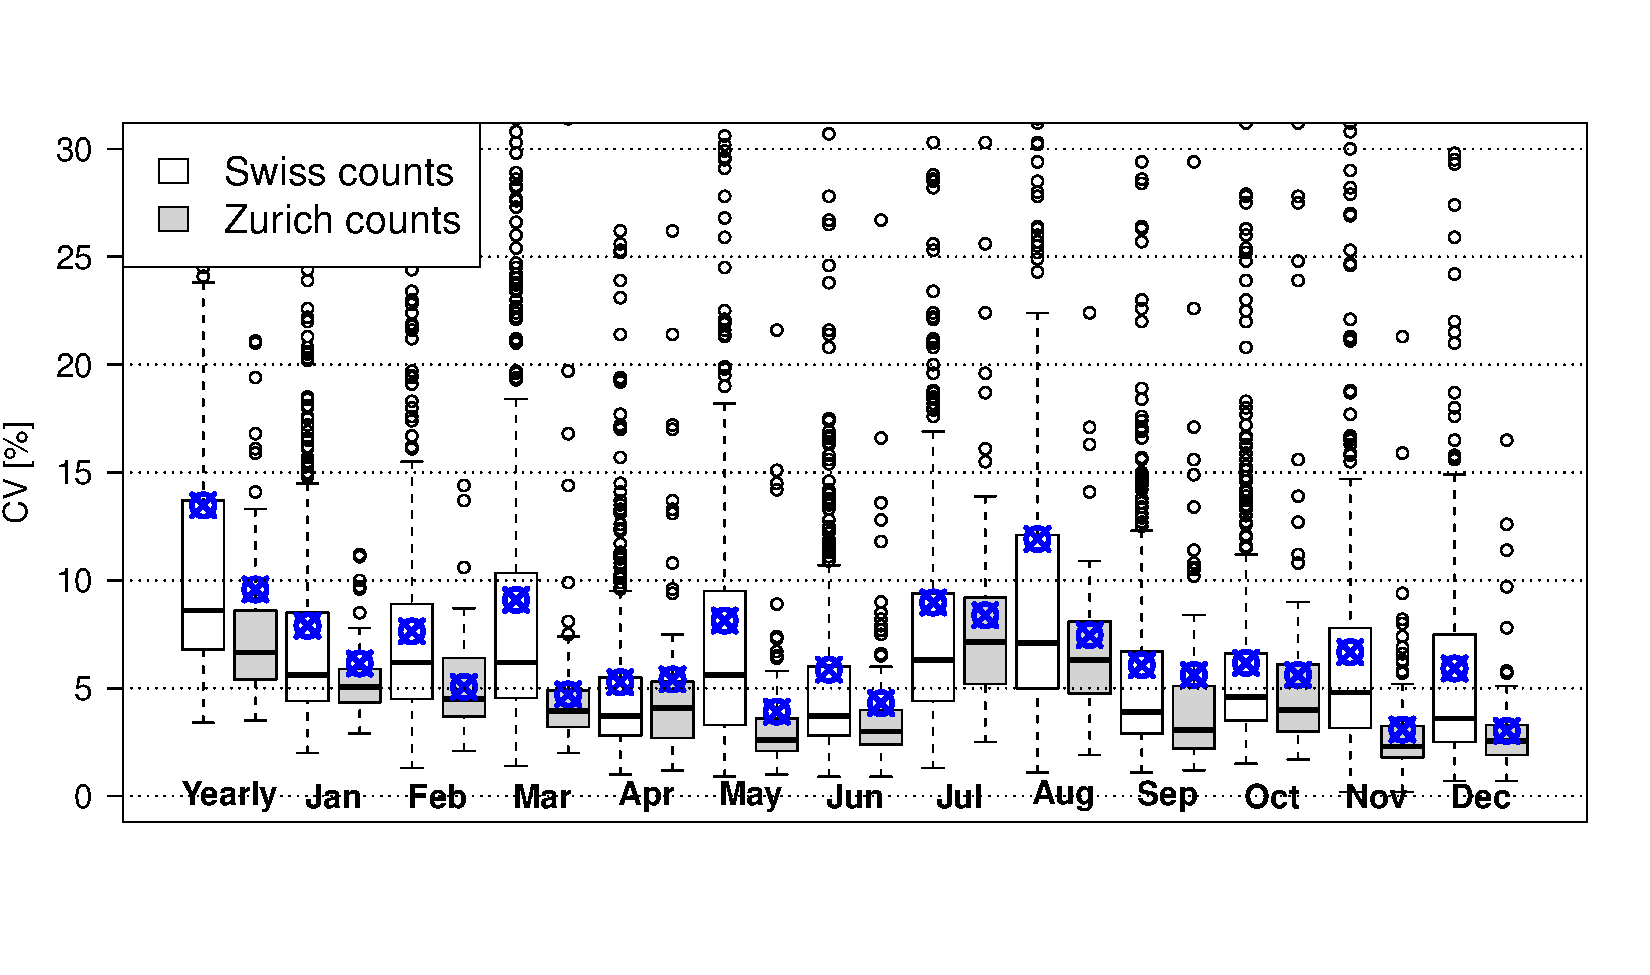
\includegraphics[height=0.3\textwidth]{understanding/figures/var/countsDaily.pdf}}%
	%{\label{fig:countsDaily}}%
  %{}%
%% ---
	%\createsubfigure%
  %{Simulated Daily Volumes: Inter-run Variability, runs~0-29, iteration~200}%
	%{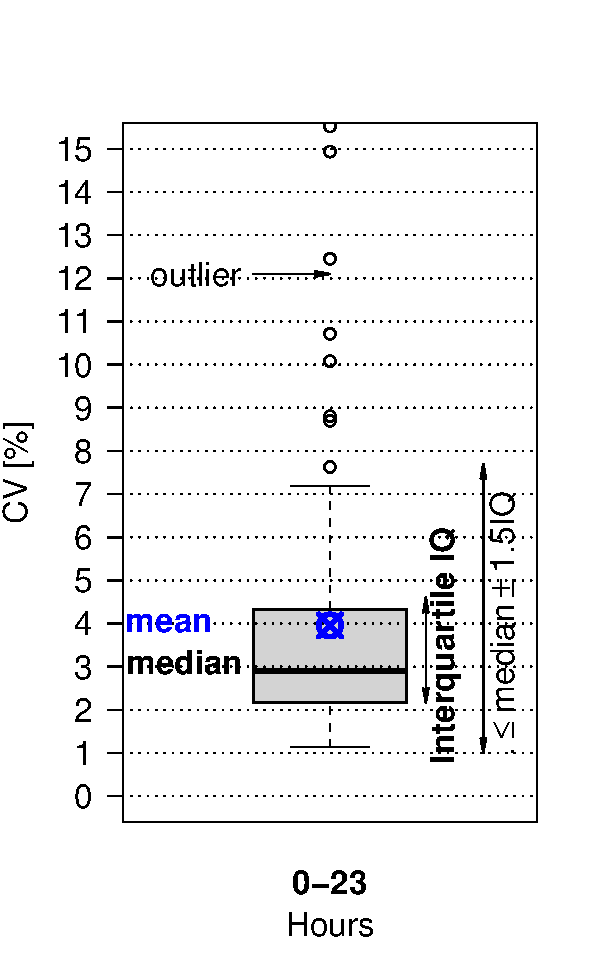
\includegraphics[height=0.3\textwidth]{understanding/figures/var/linkVolumesInterAWTV200.pdf}}%
	%{\label{fig:linkVolumesInterAWTV200}}%
  %{}%
%% ===
  %\createsubfigure%
  %{11:00-12:00}%
	%{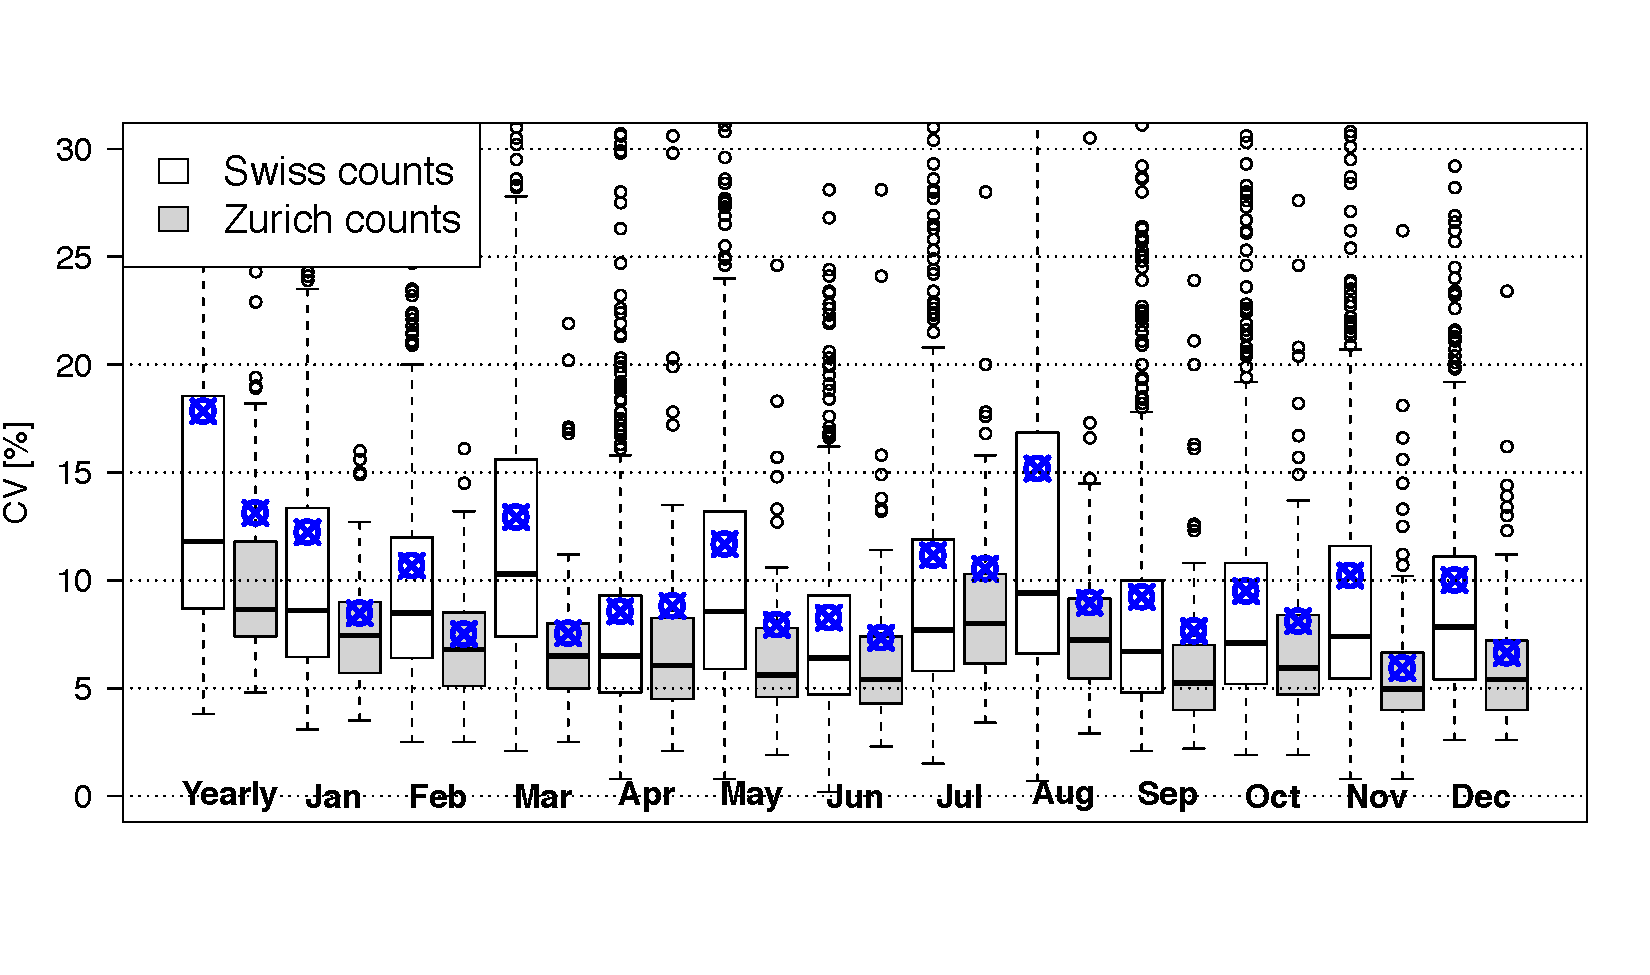
\includegraphics[height=0.3\textwidth]{understanding/figures/var/counts11-12.pdf}}%
	%{\label{fig:H1112}}%
  %{}%
%% ---
	%\createsubfigure%
  %{Simulated Hourly Volumes: Inter-run Variability, runs~0-29, iteration~200}%
	%{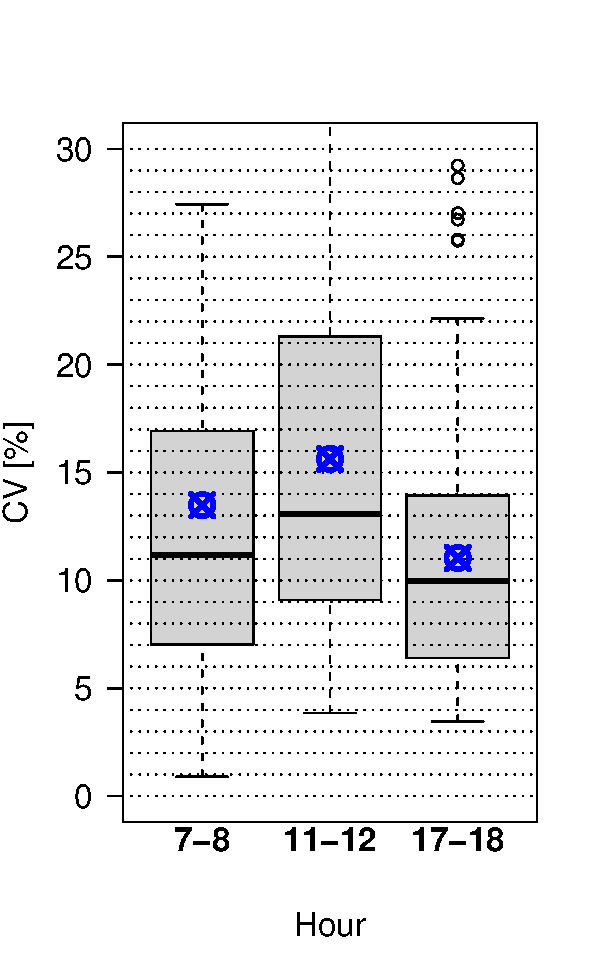
\includegraphics[height=0.3\textwidth]{understanding/figures/var/linkVolumesInter200.pdf}}%
	%{\label{fig:linkVolumesInter200}}%
  %{}%
%% ===
 	%\createsubfigure%
  %{17:00-18:00}%
	%{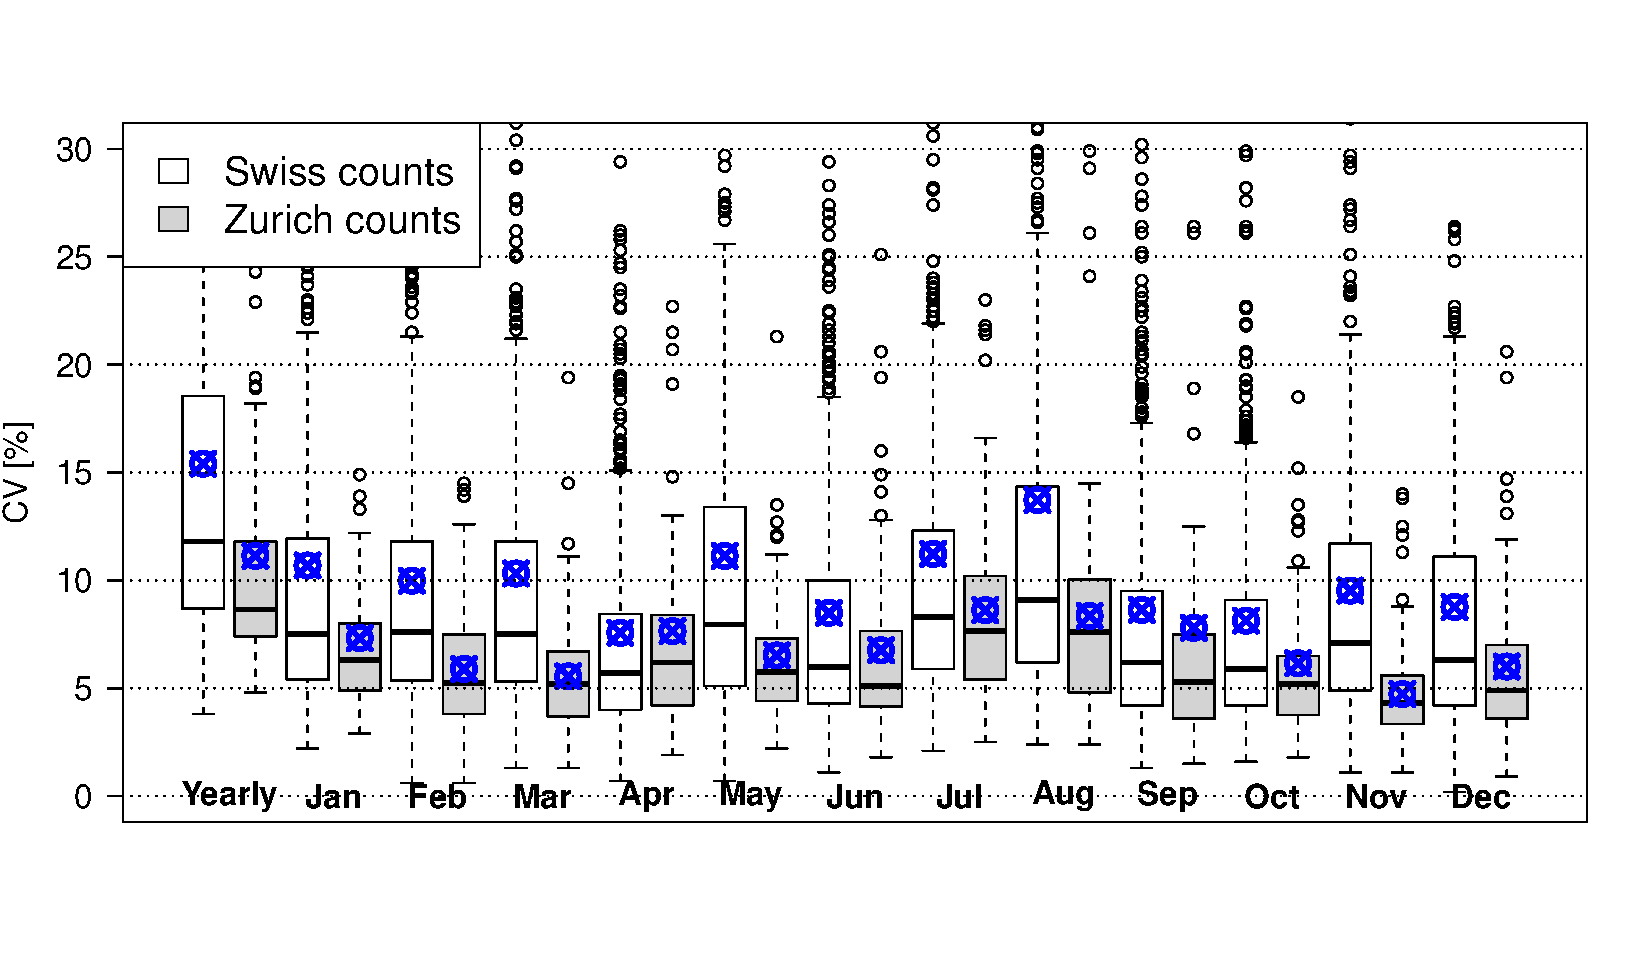
\includegraphics[height=0.3\textwidth]{understanding/figures/var/counts17-18.pdf}}%
	%{\label{fig:H1718}}%
  %{}%
%% ---
	%\createsubfigure%
  %{Simulated Hourly Volumes: Inter-run Variability, runs~0-29, iteration~200}%
	%{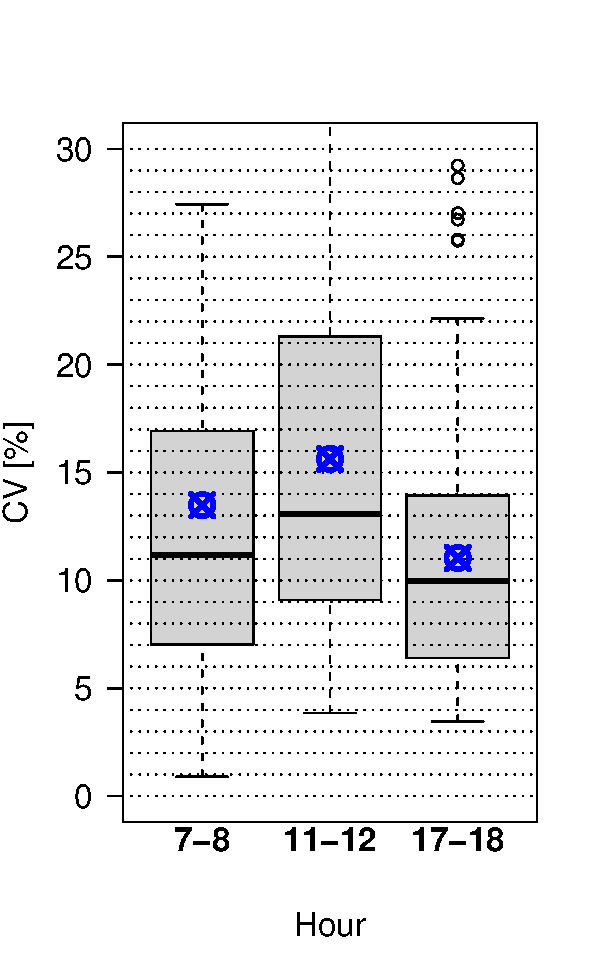
\includegraphics[height=0.3\textwidth]{understanding/figures/var/linkVolumesInter200.pdf}}%
	%{\label{fig:linkVolumesInter200}}%
  %{}%
%% ===
%}%
%{}
%
%Multiple possibilities to categorize microsimulations variability exist; some categories are described by \citet[][]{HorniEtAl_TechRep_IVT_2011_b}. Often a distinction between endogenous (model) variability and exogenous (input) variability is made. Equally suitable one can distinguish systematic and random variability. The experiments reported below mainly focus on \emph{random, endogenous} model variability. Random variability stems from inherently random choices and from actually systematic choices not recognized as systematic by the modeler.
%
%MATSim variability was investigated by \citet[][]{HorniEtAl_TechRep_IVT_2011_b, HorniEtAl_STRC_2011, Dayte_TechRep_IVT_2012} coming to the conclusion that at the population level, as expected, there is little variability between simulation results. Little variability exists likewise for \emph{daily} volumes as shown in Figures \ref{fig:linkVolumesAWTVInterScatter} and \ref{fig:linkVolumesInterAWTV200} (with a different visualization), which is consistent with previous work. However, the variability for \emph{hourly} volumes is an issue as shown in Figures~\ref{fig:linkVolumesHour17-18InterScatter} and Figure~\ref{fig:linkVolumesInter200} (with a different visualization).
%
%To interact these substantial simulation variability with variability observed in reality, \citet[][]{HorniEtAl_STRC_2011} looked at real-world link volumes given for both, the complete year and single months, meaning that a single point in the box plot represents temporal variability of a single network link, either for the whole year, or for a specific month. The hours 11-12 and 17-18 are shown as examples in Figure~\ref{fig:counts}, where similar patterns could be observed for all hours. The plots allow the conclusion that also in reality variability is also substantial.
%
%Further MATSim investigations are reported by \citet[][]{Hackney_PhDThesis_2009, Neumann_PhDThesis_2014}.
%
%\createfigure%
%{Simulated link volumes}%
%{Simulated link volumes}%
%{\label{fig:linkVolumes}}%
%{%
  %\createsubfigure%
  %{Simulated Daily Volumes: Inter-run Variability}%
	%{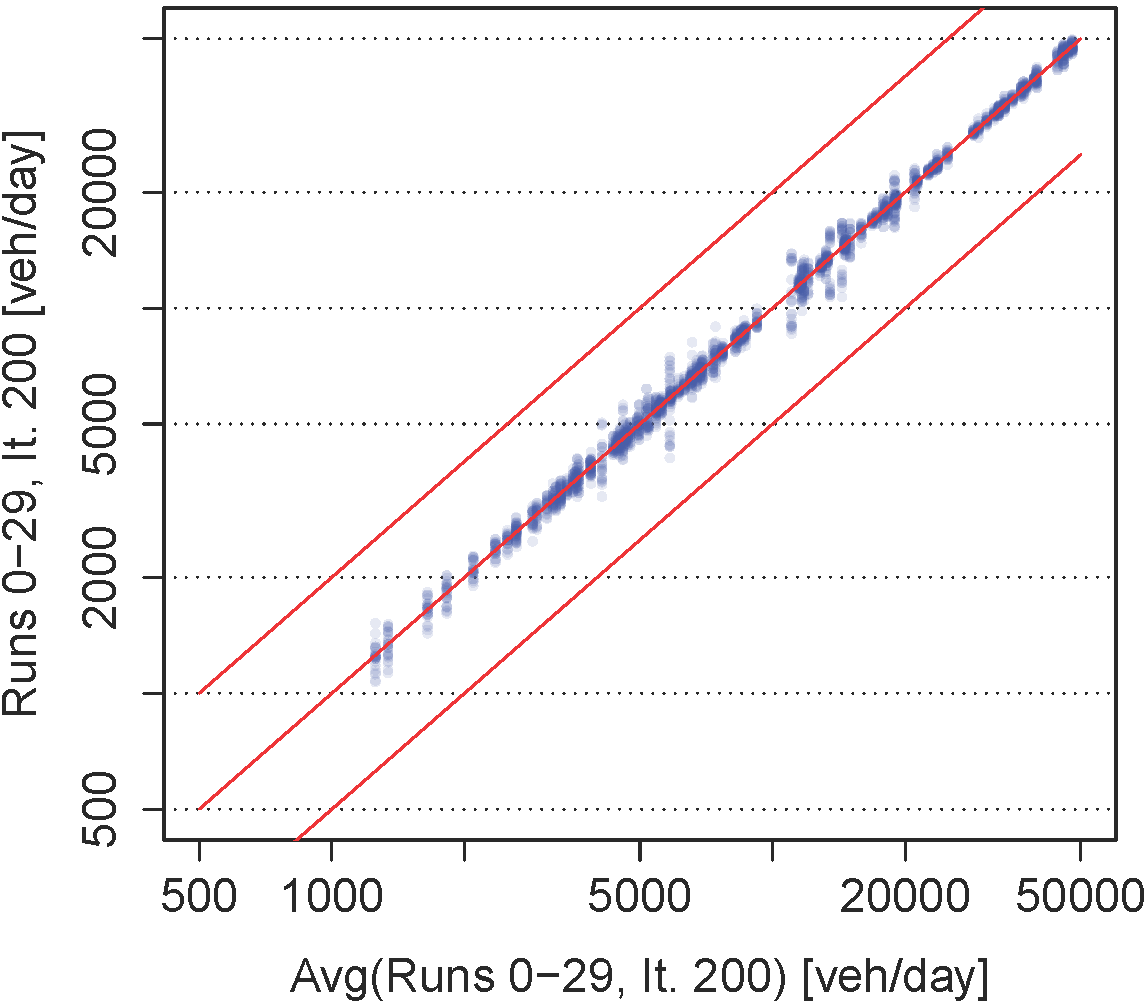
\includegraphics[width=0.49\textwidth]{understanding/figures/var/linkVolumesAWTVInterScatter.png}}%
	%{\label{fig:linkVolumesAWTVInterScatter}}%
  %{}%
	%\createsubfigure%
  %{Simulated Daily Volumes: Inter-run Variability, Runs 0-29, Iteration 200}%
	%{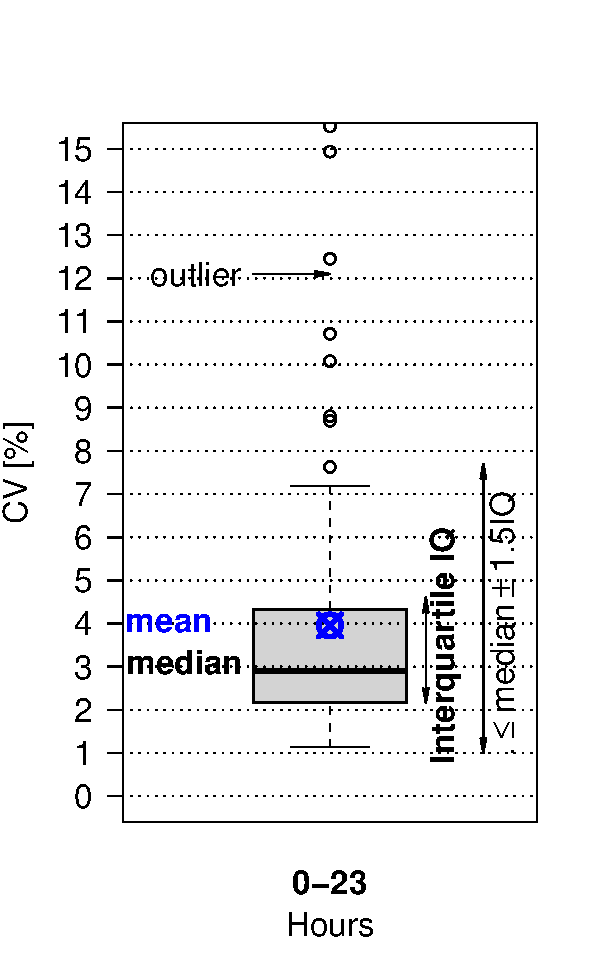
\includegraphics[width=0.3\textwidth]{understanding/figures/var/linkVolumesInterAWTV200.pdf}}%
	%{\label{fig:linkVolumesInterAWTV200}}%
  %{}%
  %\createsubfigure%
  %{Simulated Hourly Volumes (Hour 17-18), Inter-run Variability}%
	%{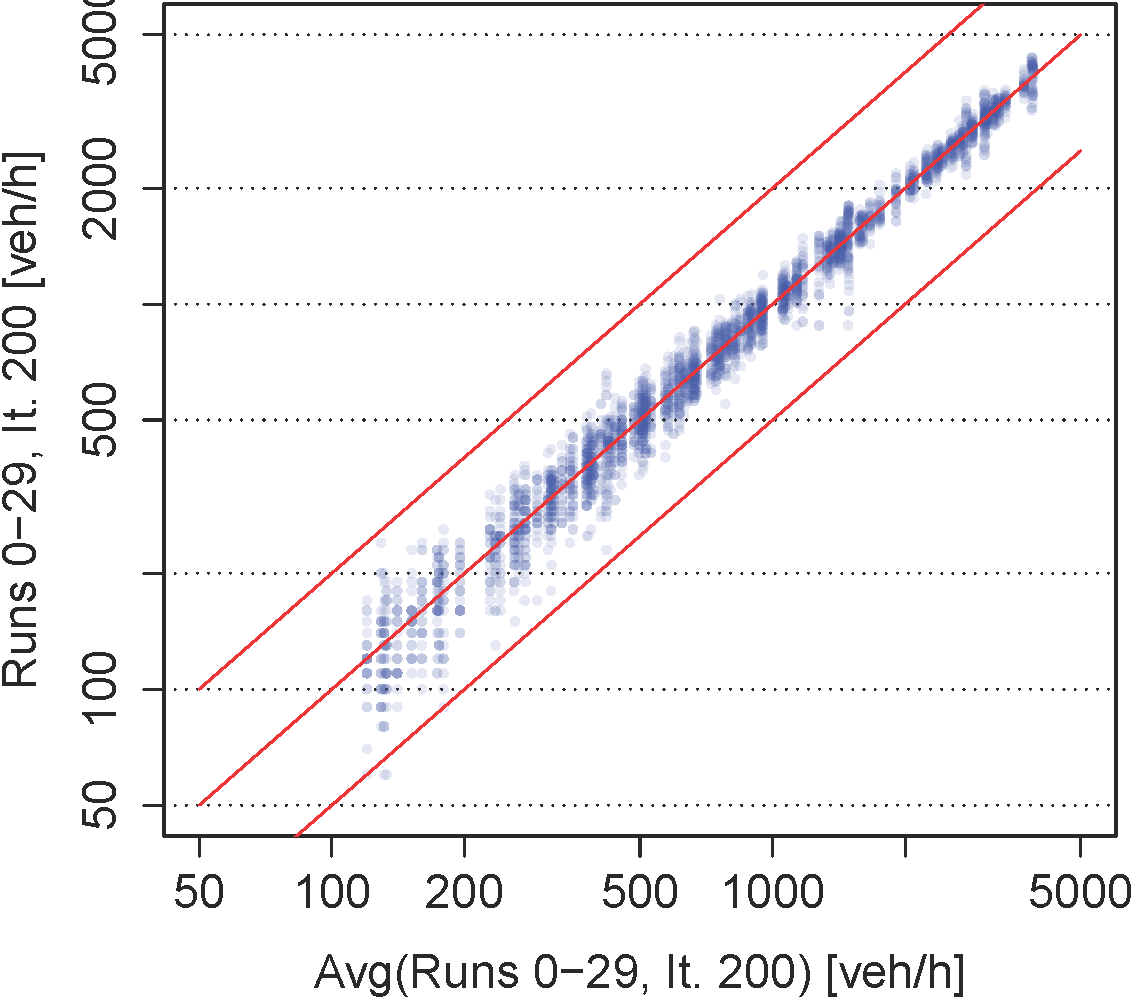
\includegraphics[width=0.49\textwidth]{understanding/figures/var/linkVolumesHour17-18InterScatter.png}}%
	%{\label{fig:linkVolumesHour17-18InterScatter}}%
  %{}%
	%\createsubfigure%
  %{Simulated Hourly Volumes: Inter-run Variability, Runs 0-29, Iteration 200}%
	%{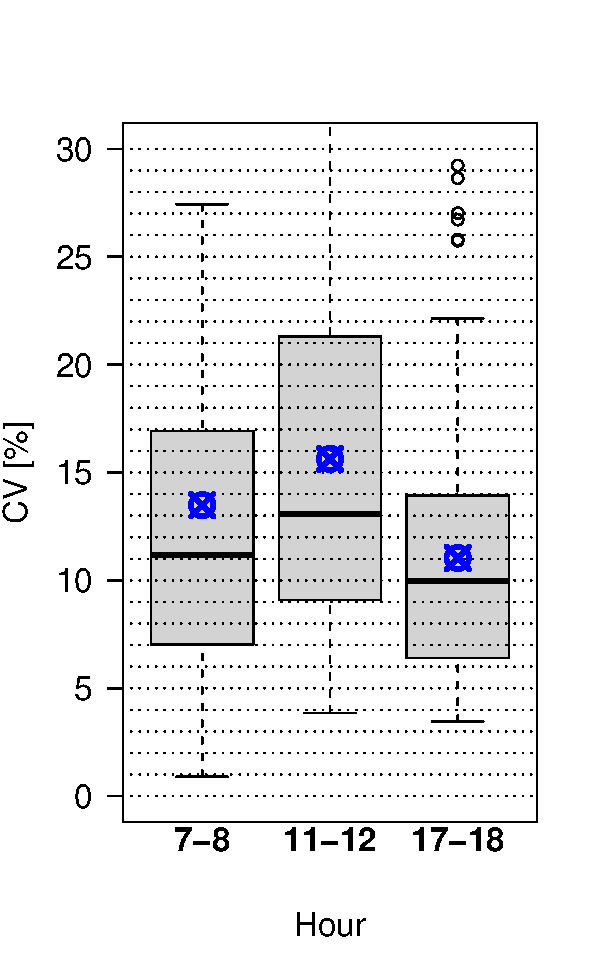
\includegraphics[width=0.3\textwidth]{understanding/figures/var/linkVolumesInter200.pdf}}%
	%{\label{fig:linkVolumesInter200}}%
  %{}%
%}%
%{} 
%
%\vfill\eject
% ##################################################################################################################
% Local Variables:
% mode: latex
% mode: reftex
% mode: visual-line
% TeX-master: "main"
% comment-padding: 1
% fill-column: 9999
% End: 
